\subsubsection{Dirbtiniai neuroniniai tinklai}

Dirbtiniai neuroniniai tinklai (angl. artificial neural networks) yra jungus tinklas, kurio viršūnės yra perceptronai, ir kurio orientuotos briaunos sujungia 2 perceptronus, iš kurių vieno perceptrono išėjimas yra naudojamas kaip kito perceptrono įėjimas. Dirbtinio neuroninio tinklo paskirtis yra spręsti klasifikavimo uždavinius.

Pagal tinklo struktūrą dirbtiniai neuroniniai tinklai yra skirstomi į tiesioginio sklidimo (angl. feedfoward)ir grįžtamojo ryšio (angl. feedback). Grįžtamojo ryšio dirbtiniai neuroniniai tinklai turi bent vieną ciklą, o tiesioginio sklidimo neturi nei vieno ciklo. Tiesioginio sklidimo neuroniniai tinklai, dėl savo paprastumo, reikalauja trumpesnio apmokymo laiko nei grįžtamojo ryšio neuroniniai tinklai. Todėl jie yra dažniausiai naudojami praktiniuose taikymuose.

Tiesioginio sklidimo tinklai yra grupuojami į vienasluoksnius perceptronus, daugiasluoksnius perceptronus ir radialinių funkcijų tinklus. Šiame darbe tiriami dirbtiniai neuroniniai tinklai, konvoliuciniai ir kapsuliniai neuroniniai tinklai, yra daugiasluoksnių perceptronų modifikacijos. Daugiasluoksnis perceptronas (angl. multilayer perceptron) yra dirbtinis neuroninis tinklas, kurio perceptronai yra sugrupuoti į sluoksnius, kuriuose gali būti skirtingas skaičius perceptronų. Kiekviename sluoksnyje esantys perceptronai turi tą pačią aktyvavimo funkciją.

Daugiasluoksnio perceptrono sluoksniai yra išsidėstę eilėje ir kiekviename sluoksnyje esančių visų perceptronų išėjimai yra tolimesnio sluoksnio visų perceptronų įėjimai. Pirmasis sluoksnis  yra vadinamas įėjimo sluoksniu ir jis susideda ne iš perceptronų, o iš mokymo duomenų vektoriaus $\boldsymbol{x}$ komponenčių. Paskutinis sluoksnis yra išėjimo sluoksnis ir jame yra tiek perceptronų kiek yra nagrinėjamų klasių, kiekvienai klasei yra priskiriamas ją atitinkantis preceptronas. Išėjimo sluoksnio perceptronų išėjimų reikšmės priklauso nuo juose naudojamos aktyvacijos funkcijos. Likę sluoksniai yra vadinami paslėptaisiais sluoksniais. Daugiasluoksnis perceptronas yra pavaizduotas paveikslėlyje \ref{img:nn}.

\begin{figure}[H]
	\centering
	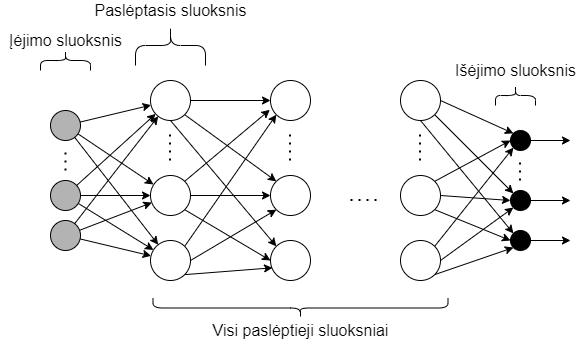
\includegraphics[scale=0.5]{img/neural_network.png}
	\caption{Daugiasluoksnis perceptronas}
	\label{img:nn}
\end{figure}

Daugiasluoksnis perceptronas pateiktam vektoriui $\boldsymbol{x}'$ priskiria klasę, kuri buvo priskirta išėjimo sluoksnio perceptronui, kurio išėjimo reikšmė buvo didžiausia iš visų išėjimo sluoksnio perceptronų.

Tam kad daugiasluoksnis perceptronas galėtų atlikti klasifikavimą, jis turi būti apmokytas. Kaip ir perceptronas, daugiasluoksnis perceptronas yra apmokomas iteratyviai keičiant visų perceptronų svorius naudojant formulę \ref{eqn:w_recalc}. Išėjimo sluoksnio perceptronams yra naudojama bendra formulė \ref{eqn:general}. Tačiau ši funkcija, paslėptųjų sluoksnių perceptronų mokymui, yra nenaudojama, nes nėra apibrėžta nuostolių funkcija $e(w)$, mat funkcijai $e(w)$ yra reikalingi perceptronų išėjimai, kurie yra nežinomi. Tad paslėptųjų perceptronų apmokymas yra vykdomas naudojant klaidos sklidimo atgal algoritmą (angl. back-propagation learning algorithm).

Klaidos sklidimo atgal algoritmas yra gradientinio nusileidimo strategijos realizacija daugiasluoksniam perceptronui. Šis algoritmo veikimo santrauka: randamas i-tosios iteracijos išėjimo vektorius $Y_i = (y_{i1}, y_{i2}, ..., y_{id})$, apskaičiuojama i-tosios iteracijos išėjimo sluoksnio perceptronų paklaidos, naudojant formulę \ref{eqn:mse_out_layer}, ir apskaičiuojami paslėptųjų sluoksnių perceptronų paklaidos, kiekvienam sluoksniui naudojant jo tolimesnių sluoksnių perceptronų paklaidas.

\begin{equation}
\label{eqn:mse_out_layer}
e_i(w) = \dfrac{1}{d}\sum_{j=1}^{d}(y_{ij} - t_{ij})^2
\end{equation}
